\chapter{Realizace subjektivních a objektivních testů}
\label{chap:realization}

\epigraph{\textit{\hfill Dvakrát měř, jednou řež.}}{-české přísloví}

K ověření předpokladu, zda objektivní algoritmy hodnotí poslechovou kvalitu nekorektně, k realizaci testů, k přípravě zvukových vzorků a k zobrazení výsledků bylo třeba využít poměrně početného programového vybavení, z jisté části ještě neexistujícího. Vzhledem ke zkušenostem autora s prostředím \matlab z dob bakalářského studia, bylo pro tyto účely využito právě toto interaktivní programové prostředí a skriptovací programovací jazyk čtvrté generace vyvíjený společností MathWorks \cite{web:matlab}. Tato kapitola popisuje jaké existující nástroje byly využity, jak byly propojeny pomocí skriptů napsaných v prostředí \matlab a jaká uživatelská rozhraní byla vytvořena pro uskutečnění poslechových testů a zobrazování výsledků.

\section{Příprava testovaného materiálu}

Před provedením jakýchkoli testů, ať už poslechových či automatizovaných, bylo potřeba připravit množinu zvukových vzorků spolehlivě reprezentující sledované parametry. To znamenalo výběr implementace kodeků, tvorbu skriptů, které je budou dávkově volat a tím generovat vzorky o různých bitových rychlostech a dalších parametrech.

\subsection{Použité kodeky}

U standardů digitálního rádia je struktura jasně definována na vysílací straně a implementace přijímače je ponechána na výrobci zařízení. Ač to může znít paradoxně, u kodeků je tomu právě naopak. Dekodér je normou důkladně popsán, zatímco kodéry mohou být napsány (či sestaveny) různě. Velké společnosti na poli audiovizuálního zpracování, jako například Fraunhoffer či Apple, si licencují vlastní (proprietární) kodéry a nechávají si za ně zaplatit poměrně velké peníze. Proto se souběžně s nimi snaží open-source komunita vytvářet kodéry vlastní. U dvou vzorků stejného profilu a stejné bitové rychlosti se tak může lišit poslechová kvalita, kvůli čemuž je důležité poznamenat jakým kodérem byl signál zakódován.

Na následujících řádcích jsou vyjmenovány implementace kodérů a dekodérů použitých v této práci.
 
\begin{itemize}
    \item TwoLame:
    
použitý ke kódování vzorků do MPEG 1 Layer II je adaptací původního freeware kodéru známého jako tooLame. Je volně dostupný z webových stránek \cite{web:twolame}. Skript \code{makeMp2} volá tento kodér napsaný v jazyce C a generuje vzorky s následujícími parametry:

    \begin{itemize}
        \item konstantní bitová rychlost (kb/s): 56, 64, 80, 96, 112, 128, 160, 192, 224, 256, 320, 384
        \item mód: stereo
        \item vzorkovací rychlost 44100 Hz
    \end{itemize}
    Pro objektivní hodnocení je ovšem nutno mít signál uložený v nezakódované formě. Vzorky tudíž byly převedeny zpět do pulzně kódové modulace pomocí programu FFmpeg \cite{web:ffmpeg}.

    \item Nero AAC Codec
    
    I u rodiny AAC byl v této práci použit freeware nástroj. Nero AAC Codec dostupný z \cite{web:nero} dokáže signál jak kódovat, tak převádět zpět do formy PCM. Dostupné profily jsou: AAC LC, HE-AAC a HE-AAC v2.
    Skript \code{makeAac} volá program \code{NeroAacEnc.exe} a vytváří vzorky s parametery:
        \begin{itemize}
        \item konstantní bitová rychlost : 12 - 256 kb/s pro profil AAC LC, 16 - 128 kb/s pro profil HE-AAC a 12 - 64 kb/s pro profil HE-AAC v2 vždy s krokem 4 kb/s.
        \item mód: stereo (pro HE-AAC v2 mód mono neexistuje, neboť využívá Parametrického sterea)
        \item vzorkovací rychlost 44100 Hz
    \end{itemize}

    \item Opus
    
    \dots je od základu vyvíjen jako open-source. Kodek je proto ke stažení přímo na stránkách standardu \cite{web:opus} a není třeba složitě shánět alternativy ve formě komunitních projektů. Podobně jako u dvou předchozích byl v matlabu vytvořen skript pro generování vzorků s následujícími parametry:
    
    \begin{itemize}
        \item konstantní bitová rychlost : 8 - 128 kb/s s krokem 4 kb/s.
        \item mód: stereo
        \item vzorkovací rychlost 44100 Hz
    \end{itemize}

    \item xHE-AAC
    
    Kódování do xHE-AAC je prozatím problematické neboť jediný současný enkodér poskytuje Fraunhoffer Institute za cenu pro komerční využití. Bylo tak třeba porozhlédnout se po zdroji zakódovaných vzorků jinde.
    Na webu DRM+ \cite{web:drm} je k dispozici ukázkové video v nezkomprimované verzi obsahující tři vzorky jak v originálu, tak zakódované pomocí xHE-AAC do dvou bitových rychlostí. Konkrétně do 8 a 12 kb/s. Pomocí programu Avidemux \cite{web:avidemux} byla z videa extrahována zvuková stopa, ze které byly programem Audacity \cite{web:audacity} vystřihány konkrétní zhruba osmi vteřinové vzorky.
    
\end{itemize}

\subsection{Typy materiálu z hlediska obsahu}
\label{subchap:material}

Doposavad se tato kapitola věnovala tomu, jak hudební vzorky zakódovat a rozkódovat. Neméně důležitým aspektem je ale skutečný obsah nahrávek použitých k testování kvality. Jelikož v éteru rádia existuje mnoho stanic vysílající různý druh obsahu od mluveného slova přes klasickou hudbu až po nezařaditelné alternativní hudební žánry, bylo třeba do palety zpracovávaných vzorků zahrnout různorodý materiál.

Tři vzorky z DRM+ videa představovaly tři kategorie, do kterých jsou nadále rozděleny všechny nahrávky figurující v této práci. Jedná se o signály:

\begin{enumerate}
    \item hudební - v indexech a skriptech značené jako \textit{music}
    \item řečové - s označením \textit{speech}
    \item smíšené - s označením \textit{mixed}
\end{enumerate}

Dalším zdrojem nahrávek byla samotná norma ITU-R BS.1387-1 \cite{itur:1387}, respektive CD přiložené k softwaru Opera \cite{web:opticom} s nahrávkami, které se používají při implementaci algoritmu PEAQ. Jedná se o izolované ukázky různých zvuků či nástrojů jako například klavír, saxofon a zpěv. V rádiu se ovšem takto osamostatněné nástroje vyskytují jen zřídka a proto z nich byl vybrán pouze jeden vzorek, konkrétně úryvek vokální skladby \textit{Tom's Diner} zpěvačky Suzanne Vega, který se ve světě multimediální techniky používá velmi často a může tak fungovat jako určitá reference vůči ostatním testům.
Zbytek nahrávek uvedených v tabulce \ref{table:material} připravil Miroslav Smutný při spolupráci na článku \textit{Perceived Audio Quality Analysis in Digital Audio Broadcasting Plus System Based on PEAQ} \cite{article:ulovecsmutny}.

\begin{table}[h]
    \centering
    \begin{tabular}{|c|c|c|c|}
    \hline
    Název vzorku & Typ & Popis & Zdroj \\ \hline
    'capriccio.wav' & Music & Úryvek klasické hudby & Smutný \\ \hline
    'holmes.wav' & Speech & Čtení z knihy Sherlock Holmes & Smutný \\ \hline
    'cimrman.wav' & Speech & Záznam hry Opeřený Had & Smutný \\ \hline
    'dubstep.wav' & Music & Elektronická hudba & Smutný \\ \hline
    'pennylane.wav' & Music & Úryvek písně od The Beatles & Smutný \\ \hline
    'refveg.wav' & Music (vocal) & A Capella zpěv & Opera \\ \hline
    'frekv3.wav' & Mixed & Řeč s hudebním podkresem & Smutný \\ \hline
    'xhedemomusic.wav' & Music & Hra na elektrickou kytaru & DRM \\ \hline
    'xhedemospeech.wav' & Speech & Úryvek řeči moderátora BBC & DRM \\ \hline
    'xhedemomixed.wav' & Mixed & Řeč s hudebním podkresem & DRM \\ \hline
    \end{tabular}
    \caption{Seznam vzorků použitých při objektivním testování kvality}
    \label{table:material}
\end{table}

Hlavně pro potřeby subjektivního testování byly za pomoci programu Audacity z nahrávek vybrány relevantní desetivteřinové úseky, které byly dále opatřeny pozvolným zesílením v první vteřině a pozvolným útlumem ve vteřině poslední.

\section{Návrh subjektivních testů}

Jak už je v úvodu naznačeno, objektivní hodnocení nahrávek zakódovaných novými kodeky využívajícími psychoakustické poznatky ve vetší míře nekoresponduje s realitou. Na tento fakt již poukazuje akademický článek \textit{Subjective and Objective Assessment of Perceived AudioQuality of Current Digital Audio Broadcasting Systems and Web-Casting Applications.} \cite{article:pocta}, kde je sledována závislost $ODG$ a $SDG$ při použití hodnotících algoritmů PEAQ a POLQA. Subjektivní testy provádí párovým srovnáváním podle \cite{itur:1116}, tedy na velké skupině expertních posluchačů. Pro potřeby této práce se ovšem lépe hodí test s vícenásobným stimulem dle \cite{itur:1534}

\subsection{Důvody pro výběr testu MUSHRA}
\begin{itemize}
    \item Zkoumaná kvalitativní oblast
    
    Protože bylo třeba ověřit zda algoritmy hodnotí věrohodně nejen tam kde je komprese nepostřehnutelná, ale skrze celé kvalitativní spektrum od výborné až po nedostatečnou, je test pro střední kvalitu podle \cite{itur:1534} mnohem vhodnější než test pro nepatrná zhoršení použitý v \cite{article:pocta}. Největší důraz bylo třeba klást na bitové rychlosti využívané v digitálním rádiu DAB/DAB+ a DRM.
    
    \item Posluchači

    Subjekty nemusí procházet sérií rozřazovacích vstupních testů. Stačí pouze zaučení přímo v grafickém uživatelském rozhraní samotného testu a doprovodné informace v přiloženém návodu (K nahlédnutí v příloze \ref{app:2}).
    
    \item Podmínky
    
    MUSHRA nemá tak přísné podmínky na provádění testu. K jeho provedení není třeba poslechová místnost s extrémně kvalitním reprodukčním zařízením. Stačí dostatečně kvalitní sluchátka a úroveň zvukového pozadí taková, aby nerušila posluchače.
    Další výhodou tohoto testu je, že lze provádět individuálně. Je tedy možné přenášet laptop se zvukovou kartou a sluchátky za subjekty a tím ušetřit čas i náklady.
\end{itemize}

\subsection{Výběr vzorků}

Jednou z nesporných výhod objektivního testování je absence únavy posluchačů, se kterou je třeba počítat při návrhu subjektivního testu. Doporučení \cite{itur:1534} říká, že délka testu by neměla překročit půl hodiny. Přímo naproti tomu jde fakt, že k zachování objektivity je třeba dostatečná diverzita poslechového materiálu. Výběr těch správných vzorků se tak stává poměrně zásadním faktorem pro výpovědní hodnotu navrženého testu.

Jak už je zmíněno v podkapitole \ref{subchap:material}. Vzorky byly rozděleny do třech kategorií. Hudební, řečové a smíšené. V druhých dvou zmíněných nedosahuje míra různorodosti vzorků takové výše jako v kategorii hudební. Vetší důraz byl tedy kladen právě na ni, a proto je v subjektivním testování zahrnuto několik vzorků reprezentujících různé hudební žánry.

Stimuly musí být, co do metody zkreslení, konzistentní skrze všechny zkoušky testu a nemožnost kódování nových zvukových záznamů do xHE-AAC tak značně zkomplikovala přípravu vzorků. Nakonec byly vytvořeny testy dva. Jeden na vyšších bitových rychlostech, obsahující všechny kodeky vyjma xHE-AAC. A druhý test na nižších datových tocích, kde společně s xHE-AAC vystupovaly zástupci novodobých kódovacích metod.

Zkoušky sestavených testů tedy obsahují vzorky uvedené v tabulce \ref{table:material:subjective}.

\begin{table}[h]
    \centering
    \begin{tabular}{|c|c|c|c|}
    \hline
    Název vzorku & Typ & Popis & Test \\ \hline
    'capriccio.wav' & Music & Úryvek klasické hudby & 1 \\ \hline
    'holmes.wav' & Speech & Čtení z knihy Sherlock Holmes & 1 \\ \hline
    %'cimrman.wav' & Speech & Záznam hry Opeřený Had & Smutný \\ \hline
    %'dubstep.wav' & Music & Elektronická hudba & Smutný \\ \hline
    'pennylane.wav' & Music & Úryvek písně od The Beatles & 1 \\ \hline
    'refveg.wav' & Music (vocal) & A Capella zpěv & 1 \\ \hline
    %'frekv3.wav' & Mixed & Řeč s hudebním podkresem & Smutný \\ \hline
    'xhedemomusic.wav' & Music & Hra na elektrickou kytaru & 2 \\ \hline
    'xhedemospeech.wav' & Speech & Úryvek řeči moderátora BBC & 2 \\ \hline
    'xhedemomixed.wav' & Mixed & Řeč s hudebním podkresem & 1,2 \\ \hline
    \end{tabular}
    \caption{Seznam vzorků použitých v subjektivních testech}
    \label{table:material:subjective}
\end{table}

\begin{table}[h]
    \centering
    \begin{tabular}{|c|C{1cm}|C{1cm}|C{1cm}|C{1cm}|C{1cm}|C{1cm}|}
    \hline
    bitrate (kpbs) & 24 & 32 & 48 & 64 & 96 & 128\\
    \hline
    Opus & \cellcolor{green!50} $\bullet$ &$\bullet$ & & & & \\
    \hline
    HE-AAC v2 & &$\bullet$&\cellcolor{green!50}$\bullet$& & &  \\
     \hline
    HE-AAC v1 & & &$\bullet$ &$\bullet$ &  &  \\
     \hline
     LC-AAC & & & & $\bullet$ & & \\
      \hline
     MPEG1 Layer II  & & & & &  $\bullet$ & $\bullet$ \\
       \hline
    \end{tabular}
    \caption{Použité bitové rychlosti v testu č. 1}
    \label{table:test1}
\end{table}

\begin{table}[h]
    \centering
    \begin{tabular}{|c|C{1cm}|C{1cm}|C{1cm}|C{1cm}|C{1cm}|}
    \hline
    bitrate (kpbs) & 8 & 12 & 24 & 48 & 64 \\
    \hline
    xHE-AAC &$\bullet$ &$\bullet$ & & & \\
    \hline
    Opus & & $\bullet$&\cellcolor{green!50}$\bullet$&  &   \\
     \hline
    HE-AAC v2 & & &$\bullet$ &\cellcolor{green!50}$\bullet$ & $\bullet$ \\
     \hline
    \end{tabular}
    \caption{Použité bitové rychlosti v testu č. 2}
    \label{table:test2}
\end{table}
Konkrétní bitové rychlosti použité v testech 1 a 2 jsou zobrazené v tabulkách \ref{table:test1} a \ref{table:test2}. Konečná volba proběhla na základě následujících kriterií: 

\begin{itemize}
    \item Bitové rychlosti používané v digitálním rádiu: 
    
    Například \textit{Advanced Audio Coding} se v systémech digitálního rádia na území České Republiky \cite{web:dab:stations} nachází ve verzích HE-AAC v1 a HE-AAC v2, tedy v základní verzi obohacené o SBR potažmo o PS. V zahraničí lze nalézt multiplexy v nichž se vysílá AAC LC profilem avšak není jich mnoho. Velký důraz je tak kladen na HE-AAC v2 profil. O něco menší na HE-AAC v1 a Low Complexity je zastoupen v testech jen jednou.
    
    \item Oblasti kde se výsledky různých algoritmů rozcházely v předběžných testech: 
    
    Například MPEG Layer II byl v předběžných testech hodnocen různými algoritmy s velkými kvalitativními rozestupy. Vzorky zkomprimované do \textit{mp2} se proto v testu nachází ve dvou bitových rychlostech.
   
    \item Výběr stejných bitových rychlostí různých kodeků k porovnání jednotlivých kompresních metod: 
    
    Kupříkladu k určení toho, jak moc velký vliv mají rozšíření SBR a PS na výslednou kvalitu.
    
    \item Sledování spíše nižších rychlostí pro určení hranice nedostatečné poslechové kvality.
    
\end{itemize}

Zeleně jsou zvýrazněny vzorky, ve kterých se testy vzájemně překrývají.

%\begin{comment}
\subsection{Použité vybavení}

Provést subjektivní testy v poslechové místnosti velkou skupinou posluchačů se ukázalo jako časově a hlavně koordinačně velmi náročné. Byla proto zvolena varianta testu přenosného, který lze realizovat kdykoliv a kdekoliv, kde není přítomno zvukové rušení. Testy byly spouštěny přímo v prostředí \matlab bežícím na čtrnácti palcovém notebooku ThinkPad E431. Jako poslechové zařízení byla použita studiová sluchátka, používaná na katedře Radioelektroniky fakulty Elektrotechnické ČVUT k poslechovým testům v rámci výuky zvukové techniky. Konkrétně šlo o model Sennheisser HD 200 PRO. Parametry udávané výrobcem jsou v tabulce \ref{table:hd200}. 

\begin{table}[h]
    \centering
    \begin{tabular}{|c|c|}
    \hline
    Harmonické zkreslení (THD): & \textless{}0,1 \% \\ \hline
    Jmenovitá impedance: & 32 Ohm \\ \hline
    Délka kabelu: & 2 m \\ \hline
    Frekvenční rozsah: & 20 - 20 000 Hz \\ \hline
    Hmotnost: & 184 g \\ \hline
    Konstrukce: & uzavřená, dynamická \\ \hline
    Akustický tlak: & 108 dB ( 1 Vrms ) \\ \hline
    \end{tabular}
    \caption{Parametry  sluchátek Sennhesier HD 200 PRO udávané výrobcem \cite{web:senn}}
    \label{table:hd200}
\end{table}

Zda frekvenční charakteristika sluchátek odpovídá přísné toleranční masce podle ITU-R BS.708 \cite{itur:708} bylo ověřeno měřením na umělém uchu Brüel \& Kjær 4153 \cite{web:earsim}. Blokové schéma zapojení se nachází na obrázku \ref{pic:measure}.

\begin{figure}[h]
    \centering
    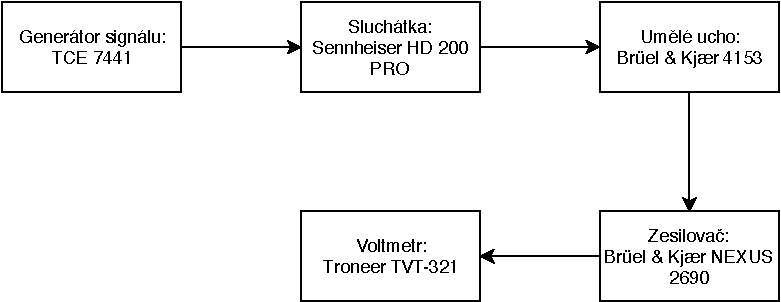
\includegraphics[width = .8\textwidth]{pic/measure.pdf}
    \caption{Blokové schéma zapojení měřícího pracoviště při měření sluchátek Sennhesier HD 200 PRO}
    \label{pic:measure}
\end{figure}

 Naměřená frekvenční charakteristika je na obrázku \ref{pic:hd200}. V nejvyšší části basového pásma a nejnižší oblasti středních kmitočtů nesplňuje přísné hranice masky ITU-R. Sluchátka nicméně byla použita s přihlédnutím k následujícím kritériím.
 
 \begin{itemize}
     \item Doporučení ITU-R BS.1534 MUSHRA se na kvalitu sluchátek odvolávají skrze normu ITU-R BS.1116 pro měření nepatrných zhoršení. Testování v rámci této práce se však zabývá střední kvalitou. 
     \item Frekvenční charakteristika sluchátek Sennheiser HD 280 PRO, která podle webové stránky rtings.com \cite{web:rtings}, věnující se podrobnému měření studiových sluchátek, dosahuje velmi podobného zvlnění a vybočuje tak z masky dané doporučením BS.708 stejně jako Sennheiser HD 200 PRO. I přes to jsou sluchátka HD 280 PRO použita v následujících akademických pracích, které taktéž k hodnocení kvality využívají test MUSHRA.
     \begin{itemize}
         \item \textit{Considering Bluetooth's Subband Codec (SBC) for Wideband Speech and Audio on the Internet} \cite{headphones1} - článek nalezený na webu \textit{Researchgate.com} zabývající se problematikou kódování širokopásmového zvuku pro přenos internetovým rádiem.
         \item \textit{Acoustic echo reduction robust against echo-path change with instant echo-power-level adjustment} \cite{headphones2} - článek nalezený na webu \textit{ieeexplore.com} který se zabývá odstraňováním dozvuku v telekomunikacích.
     \end{itemize}
 \end{itemize}

\begin{figure}[h]
    \centering
    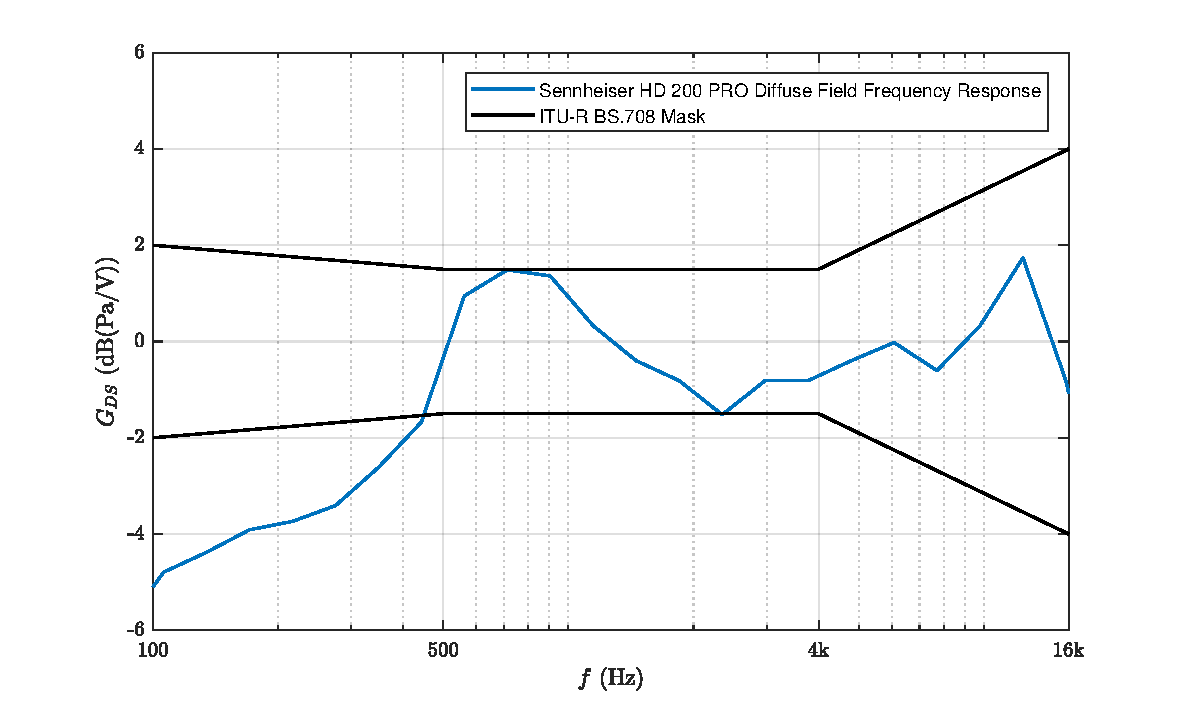
\includegraphics[width = \textwidth]{pic/headphones.pdf}
    \caption{Frekvenční charakteristika sluchátek Sennhesier HD 200 PRO změřená na umělém uchu Brüel \& Kjær}
    \label{pic:hd200}
\end{figure}


K převodu na analogový signál byla použita externí zvuková karta AxagonHQ ADA-HP, jejíž relevantní technické parametry udávané výrobcem jsou uvedeny v tabulce \ref{table:soundcard}. Hladina okolního šumu nebyla při provádění testu měřena, nicméně byl kladen důraz na to, aby ruch okolí nerušil subjekty při poslechu.

\begin{table}[h]
    \centering
    \begin{tabular}{|c|c|}
    \hline
    Analogový výstup & \begin{tabular}[c]{@{}c@{}}2kanálový stereo výstup pro sluchátka \\ nebo aktivní reproduktory\end{tabular} \\ \hline
    Vzorkovací frekvence & 44.1 / 48 / 96 kHz analog \\ \hline
    Rozlišení & 16 / 24 bit pro přehrávání \\ \hline
    Odstup signál / šum & $\geq$ 95dB (Output SNR) pro DAC \\ \hline
    Harmonické zkreslení & $\leq$ -85dB (Output THD+N) \\ \hline
%    Konektor & 3.5 mm stereo jack (sluchátkový výstup) \\ \hline
%    Rozhraní & USB 2.0 / USB 1.1 \\ \hline
    \multicolumn{1}{|l|}{Sluchátkový zesilovač} & \multicolumn{1}{l|}{\begin{tabular}[c]{@{}l@{}}20 - 20.000 Hz, výkon 105 mW / 16 ohm,\\  při 1kHz 0.1\% THD+N, 16 - 100 $\Omega$\end{tabular}} \\ \hline
    \end{tabular}
    \caption{Parametry zvukové karty AxagonHQ ADA-HP udávané výrobcem \cite{web:axagon}}
    \label{table:soundcard}
\end{table}

\subsection{Grafické uživatelské rozhraní}

Jelikož MUSHRA test se využívá k poslechovým testům více než deset let, existují již před-připravené skripty a programy do kterých stačí naimportovat vzorky a není třeba se zabývat programováním GUI a vyhodnocovacích algoritmů. Většina takových programů je ovšem zatížena licenčními polatky. Vedle komerčních produktů existují i komunitou psané freeware programy jako jsou WhisPER\cite{article:whisPER}, APE\cite{article:APE} a Scale. 

Po zvážení byl vybrán právě program Scale \cite{article:scale} připravený pro použití v jazyce \matlab. Jeho předností by měla být implementace rozhraní pro provádění všech testů popsaných v kapitole \ref{chap.listeningTests}. Kromě samotného testu se pyšní i schopností výsledky vyhodnotit.

Po několika pokusech využít Scale se ovšem začaly objevovat problémy. Při větším množství vzorků nahraných do rozhraní MUSHRA prostředí \matlab hlásilo chyby, vyhodnocování bylo spolehlivé pouze pro test pro nepatrná zhoršení \cite{itur:1116} a jednodušší než opravovat existující program se začalo zdát napsat si program od základu.

%\subsection{Zvolené prostředí}

Pro návrh grafického uživatelského rozhraní se v matlabu nachází komponenta GUIDE \cite{web:guide}. Jedná se o nástroj, ve kterém se pomocí kurzoru myši dají rozmístit objekty z nabídky do prostoru okna, které se poté oživují psaním funkcí zvaných \textit{callbacks}. Ty jsou vyvolány akcemi jako například kliknutím myši, či stiskem klávesy. Objekty jsou definovány souborem vlastností uložených ve speciálním datovém typu \textit{handle} a jdou dle potřeby vyčítat či upravovat obdobně jako standardní datové proměnné v klasických funkcích. Na následujících řádcích je stručně popsáno výsledné rozhraní, ve kterém byly testy MUSHRA realizovány.

\begin{itemize}
    \item Uvítací okno
    
    Jednoduché GUI s rámcovým popisem testu, dvěma dialogy pro zadání jména a věku subjektu a tlačítkem pro přechod do další fáze testu. Uvítací okno je k vidění na obrázku \ref{pic:intro}.
    
    \begin{figure}[h]
        \centering
        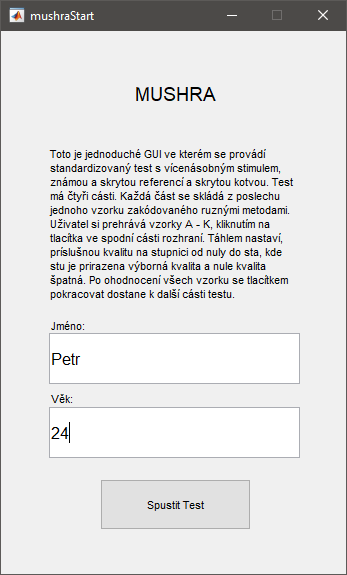
\includegraphics[width=.32\textwidth]{pic/intro.png}
        \caption{Grafické rozhraní uvítacího okna}
        \label{pic:intro}
        \end{figure}
        
        \item Zaučení
        
        Okno velmi podobné \uv{ostrému} testování. Na rozdíl od něj zde nejsou vzorky seřazeny náhodně, ale pod každým tlačítkem se nachází zvuková nahrávka odpovídající popisu v pravé části okna. Uživatel si takto může jednotlivé typy stimulů projít a naučit se, co je to \uv{kotva}, \uv{skrytá reference} a na jaké druhy zkreslení může při testu narazit.

\begin{comment}
    \begin{figure}[h]
    \centering
    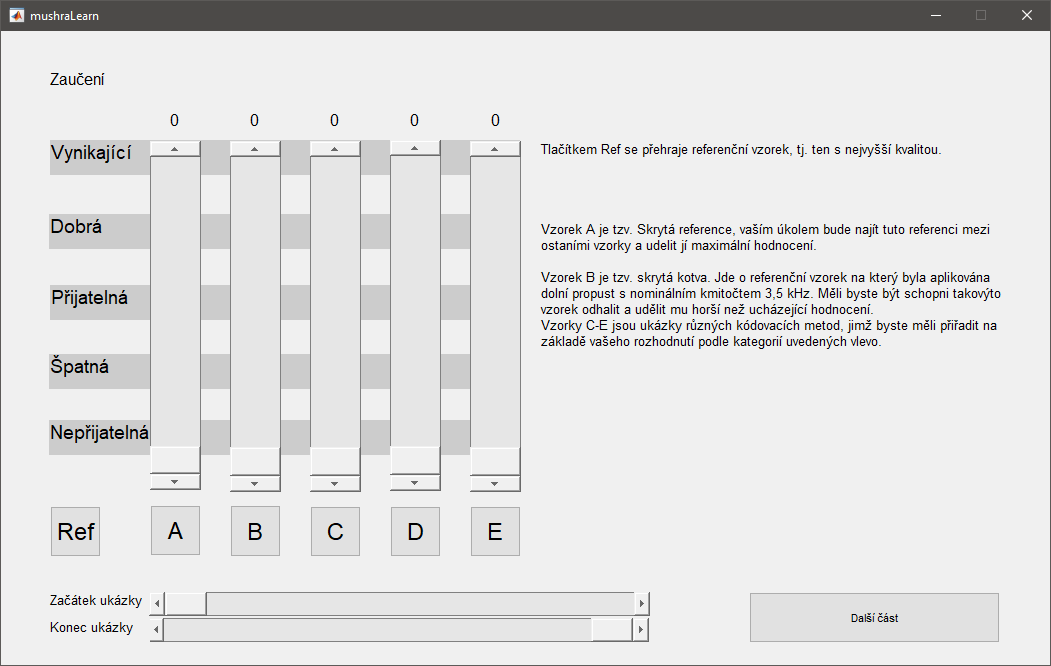
\includegraphics[width=.75\textwidth]{pic/learn.png}
    \caption{Grafické rozhraní části zvané: Zaučení}
    \label{pic:learn}
    \end{figure}
\end{comment}    

    \item Okno pro jednu zkoušku testu
    
    
Toto okno se přizpůsobuje na základě toho jaký návrhář testu zvolí počet zkoušek a vzorků. Soubor \code{scenarios.txt} v kořenovém adresáři testu, obsahuje názvy jednotlivých zkoušek oddělených novým řádkem. Pro představu test popsaný v tabulce \ref{table:test1} je zapsán takto:

\samepage{\code{Klasická hudba\\
Rock\\                            
Mluvené slovo\\
Zpěv(acapella)\\
Mixed}}

Tomu musí odpovídat počet podsložek uložených do složky \code{scenarios}. Podle počtu vzorků v podsložkách se aktivuje počet přehrávacích tlačítek hodnotících posuvníků. Maximálně jich ovšem může být 12 včetně dvou referencí a jedné kotvy.

Nad každým posuvníkem se nachází udělené hodnocení v procentech. Pro lepší orientaci jsou posuvníky podkresleny barevně odlišenými oblastmi, které odpovídají kvalitativním úrovním definovaným v doporučení ITU-R BS 1534.

Po vyplnění všech zkoušek je test ukončen dialogovým oknem s nápisem \uv{Konec!}, které volá funkci pro export výsledků do souboru.

O průměrování, post-screening a zobrazení do sloupcových grafů se stará skript \code{displayResults}, taktéž umístěný v kořenovém adresáři testu.

\begin{figure}[h]
\centering
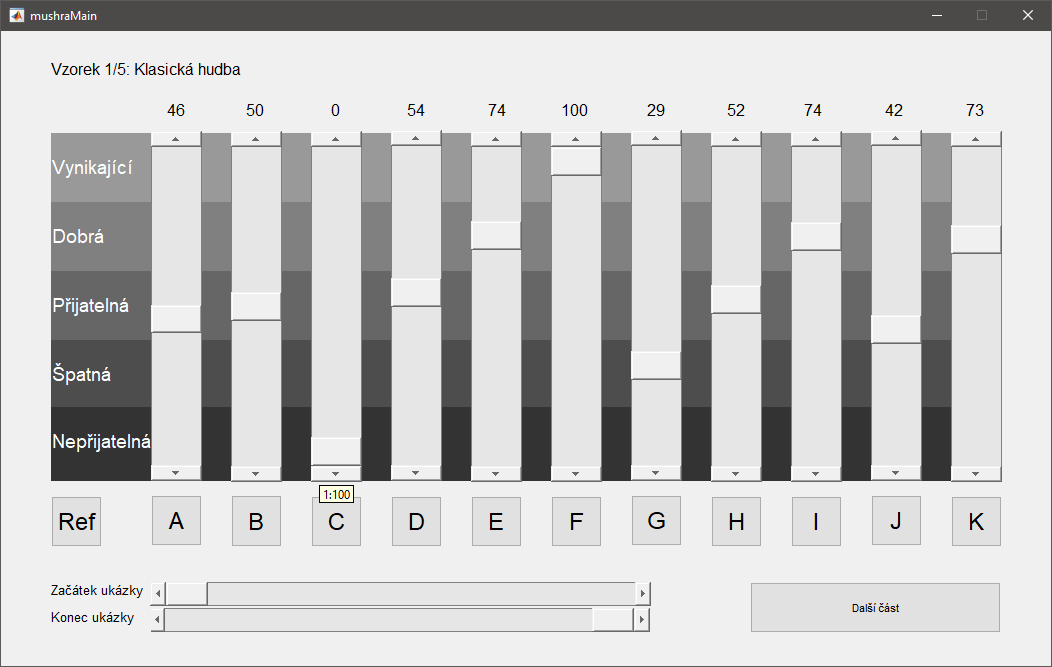
\includegraphics[width=.95\textwidth]{pic/test.png}
\caption{Grafické rozhraní průběhu testu}
\label{pic:test}
\end{figure}

Posuvníky ve spodní části okna nazvané \uv{Začátek ukázky} a \uv{Konec ukázky} slouží k časovému omezení všech přehrávaných vzorků dané zkoušky. Touto funkci lze využít při rozhodování pouze na základě krátkého úseku vzorku. Například při podezření, že se v ukázce vyskytuje kompresní artefakt.


\end{itemize}

\section{Použité implementace algoritmů pro objektivní testování kvality audiosignálů}

\subsection{PEAQ}

Matlabová implementace PQevalAudio základního modelu PEAQ je volně k dispozici na stránkách univerzity McGill \cite{web:mcgill}. V předběžných testech byl využit právě tento model, nicméně sami autoři v poznámkách tvrdí, že slouží pro výukové účely a nikoliv pro výzkum na poli zvukového zpracování, jelikož nesplňuje všechna kritéria vytyčená doporučením \cite{itur:1387}. Proto se v praxi se základní verzí algoritmu příliš nesetkáváme. Pokročilá verze byla implementována v roce 2003 do programu s názvem Opera\footnote{Opera obsahuje i základní verzi algoritmu PEAQ.} německou firmou OPTICOM \cite{web:opticom}, která se soustředí na vývoj softwaru pro hodnocení kvality zvuku již od roku 1995 a podílela se i na vzniku standardu \cite{itur:1387}. Katedra radiotechniky ČVUT má zakoupenou licenci tohoto programu pro akademické využití. K ověření platnosti licence využívá USB klíčenku, kterou je třeba mít připojenou k PC po celou dobu běhu algoritmu.

Rozhraní programu (na obrázku \ref{pic:Opera}) je poměrně spartánské. V levém horním rohu se nachází tlačítka pro obsluhu. Zbytek prostoru je vyhrazen pro prezentaci výsledků hodnocení. Tlačítkem \uv{Start} s obrázkem vlaječky se spouští průvodce importem vzorků. Lze použít různé mapování kanálů, kompenzaci zpoždění, a několik filtrů, například odstranění stejnosměrné složky.

Po zadání všech parametrů a cest k referenčnímu a testovanému vzorku přejde program k hodnocení a po dokončení běhu algoritmu zobrazí výsledky jako například: zpozdění, rozdíl hlasitostí vyjádřený v úrovních, délky vzorků a především $ODG$ s grafickou reprezentací.

\begin{figure}[h]
    \centering
    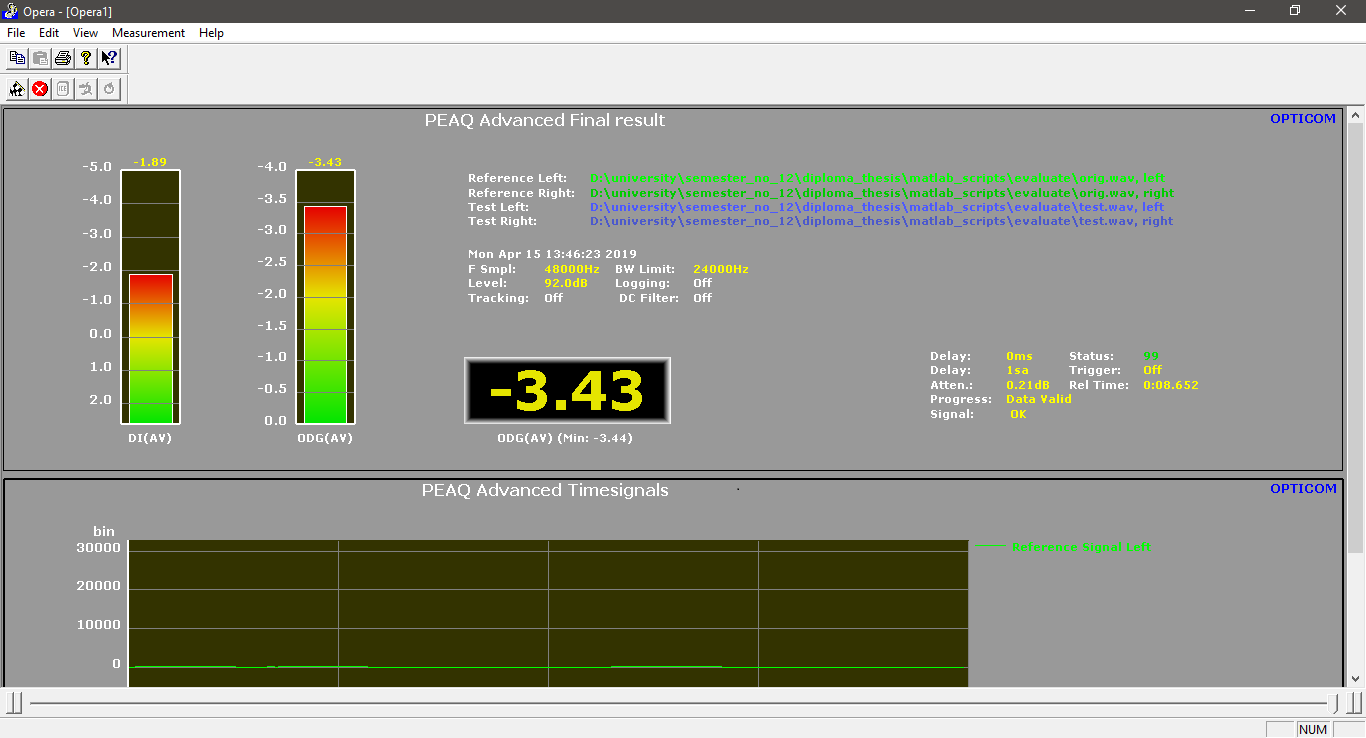
\includegraphics[width=.95\textwidth]{pic/opera.png}
    \caption{Uživatelské rozhraní programu OPERA}
    \label{pic:Opera}
\end{figure}


Takovýto postup je časově náročný a při hodnocení stovek až tisíců vzorků nepoužitelný. Naštěstí lze Opera volat z příkazové řádky a tím je proces automatizovatelný. Volání programu \code{opera.exe} vrací záznam ve formě tabulky v textovém souboru, ze kterého lze parametry předat jiným programům.

I přes to, že se v akademické sféře používá pokročilý model, čistě ze zvědavosti autora jsou v této práci zahrnuty výstupy obou verzí algoritmu počítané programem Opera.

\subsection{PEMO-Q}

Balík \code{OpenQual+} vznikl jako přepis implementace algoritmu PEMO-Q z diplomové práce Martina Zalabáka \cite{thesis:zalabak} užitím principů objektově orientovaného programování. Zároveň je kód upravený tak, aby poskytoval výsledky blížící se verifikované komerční implementaci PEMO-Q od HörTech gGmbH \cite{web:hortech}. Jeho autor Jan Novák ve své bakalářské práci \cite{thesis:novak} zmiňuje, že balík je optimalizovaný pro \matlab 2017a a novější. Ve verzi 2018b nicméně vykazoval značně podivné chování často končící chybou, což je důvod proč je v této práci použito právě prostředí 2017a i přes svou téměř dvou roční zastaralost. Smyslem objektově orientovaného přístupu při programování \code{OpenQual+} byla myšlenka jednoduché rozšířitelnosti o další hodnotící algoritmy. V této práci je ovšem využita pouze pro hodnocení metodou PEMO-Q.

Inicializace balíku probíhá skrze metodu \code{ getEvaluationEngine}, která po zadání parametrů vrátí instanci třídy modelu, se kterým se dá následně pracovat jako s obyčejnou funkcí pomocí příkazu \code{ engineInstance.evalObjQuality(y,y1)}, kde \code{y} je referenční vzorek a \code{y1} je vzorek testovaný.
Ve srovnání s programem Opera je hodnocení poměrně časově náročné.

\subsection{ViSQOL Audio}

Zprovoznění implementace algoritmu ViSQOL bylo ze všech použitých implementací nejjednodušší. Jedná se o funkci \code{visqol.m} napsanou v jazyce \matlab dostupnou z \cite{web:visqol} se vstupy pro referenční signál, testovaný signál a parametry. Těmi je konkrétně myšleno, zda bude použit základní model pro hodnocení hlasu či pokročilý ViSQOL-Audio.

Jelikož původně byl algoritmus ViSQOL vyvíjen k hodnocení kvality přenosu řeči v telekomunikacích, neposkytuje výsledky ve formě $ODG$, ale na škále \textit{MOS-LQO} (\textit{Mean Opinion Score - Linear Quadrature Objective}). Je to taktéž jediný výstup funkce \code{visqol.m}, což může být bráno jako nevýhoda oproti algoritmům PEAQ a PEMO-Q, které disponují větším množstvím výstupních parametrů.
\begin{comment}
    V doporučení \cite{itur:1284} v kapitole 5: \textit{Grading Scales}, je tabulka (uvedená na obrázku \ref{pic:mosodg}), která pokládá pomyslné rovnítko mezi stupnice \textit{MOS} a $ODG$. 
    
    \begin{figure}[h]
        \centering
        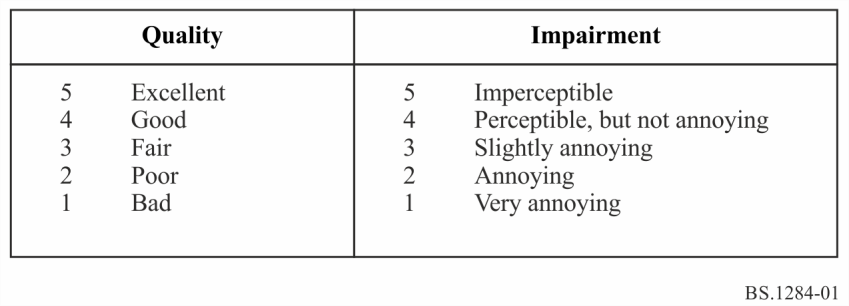
\includegraphics[width=0.7\textwidth]{pic/mos_odg.png}
        \caption{Vztah $MOS$ a $SDG$ ($ODG$) z \cite{itur:1284}}
        \label{pic:mosodg}
    \end{figure}
\end{comment}


\section{Popis ostatních funkcí, skriptů a rozhraní}

V průběhu této diplomové práce bylo připraveno v rozhraní \matlab několik skriptů, funkcí a programů, jenž slouží ke generování vzorků, jejich hodnocení a zobrazování výsledků. V následujících podkapitolách je popsána jejich funkce a ovládání.

\subsection{main}

Main je skript propojující většinu funkcí, skriptů a podprogramů, použitých při vyhodnocování kvality zvuku. Jeho kompletní kód je v digitální příloze.% \ref{code:main}.
Postupně se na základě uživatelského vstupu stará o:
\begin{itemize}
    \item inicializaci cest
    \item přípravu zakódovaných souborů
    \item hodnocení objektivními algoritmy
    \item zobrazení výsledků
\end{itemize}

\subsection{evaluate}

Funkce \code{evaluate} provádí sekvenčně několik operací. Na základě vybraného kodeku přidělí možné bitové rychlosti, ve kterých je hodnocení možné. Následně načte testovaný vzorek, k němu ve složce \code{original} vyhledá referenci a vyřeší časové zarovnání, bez něhož by hodnocení nebylo korektní. Poté oba vzorky předá hodnotícímu algoritmu, popřípadě provede převzorkování na jiný kmitočet, a výsledné hodnocení uloží do souboru pro další zpracování.

\subsection{showResults}

Grafické rozhraní \code{showResuls} slouží k prezentaci závislostí $ODG$ na bitové rychlosti, získaných z výstupů objektivních algoritmů pomocí funkce \code{evaluate}. K návrhu byl využit systém GUIDE \cite{web:guide}. Okno programu na obrázku \ref{pic:showResults} je rozdělené do dvou částí. Vlevo se nachází ovládací prvky, vpravo je prostor pro zobrazení grafů. Vykreslení grafů reaguje okamžitě na uživatelem volenou kombinaci kodeků (přepínačem \textit{Codec}) a hodnotící metody (přepínačem \textit{Method}). Tlačítkem \textit{Choose Samples} se otevře dialogové okno \code{ChooseDialog}, ve kterém je možné vybrat si pouze vzorky, jenž uživatele zajímají. Přepínačem \textit{Display} lze vykreslit celou množinu závislostí, či jejich aritmetický průměr společně se směrodatnou odchylkou.
Hodnoty na ose \textit{x} lze buďto nechat automaticky se přizpůsobovat obsahu grafu, nebo lze zatrhávacím boxem \textit{Fixed Bitrate} zvolit pevný rozsah v intervalu $\langle12;384\rangle$ kb/s.

\begin{figure}[h]
\centering
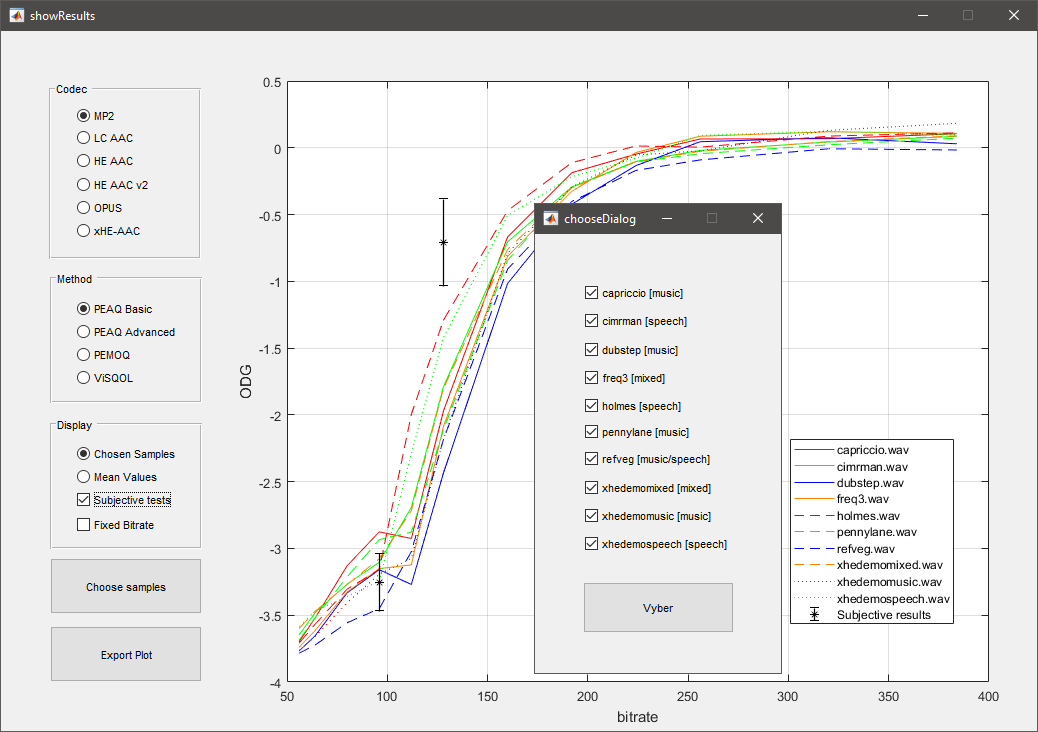
\includegraphics[width=.85\textwidth]{pic/showResults.png}
\caption{Grafické rozhraní \code{showResults}}
\label{pic:showResults}
\end{figure}

Zatrhávací box \textit{Subjective tests} umožňuje zobrazit výsledky subjektivních testů, pokud jsou k dispozici. Protože rozhraní \code{showResults} bylo vymyšleno pro vykreslování výsledků hodnocení objektivními algoritmy, je tato funkce pouze doplňková a nectí set vybraných vzorků tlačítkem \textit{Choose Samples}, který ostatně vůbec nemusí být shodný.  Při kliknutí myší na tento box se zobrazí varování o tom, na kterých vzorcích byl subjektivní test proveden. Je ponecháno na uživateli, aby dbal na to jaká data porovnává. 
Grafy lze exportovat tlačítkem \textit{Export Plot} do formátů pdf, png, jpeg a bmp..

\subsection{makeCell}

Výsledky objektivního hodnocení je do zobrazovače \code{showResults} třeba importovat. Skript \code{makeCell} je jednoduchý kód jehož úkolem je kumulace výsledků (závislostí $ODG$ na bitových tocích) z funkce \code{evaluate} do jednoho souboru, se kterým se bude lépe pracovat. V Matlabu pro takové aplikace existuje datový typ zvaný buňka (\textit{cell}), do kterého jdou nořit libovolné datové typy. Buňka
vytvořená pomocí funkce \code{makeCell} má následující kořenovou strukturu:

\centerline{\code{cellName/algorithms/codecs/odgs}}

